\section{Planning}
\subsection{Group Breakdown}
When dividing work up among the group members, all involved will contribute to all aspects of the project. Technical leads have been established for the various facets of the project to ensure needs are evenly addressed and guide overall direction for tasks. The individual in charge of a given task will not work alone on the task, rather, they ensure the needs of the task are being addressed via combined contributions from all group members. 
\begin{itemize}
\item \textbf{Benjamin Rudson}: Project Lead, responsible for managing the overall project timeline, in particular ensuring that all triple bottom line concerns have been addressed. 
\item \textbf{Andrew Cantanna}: R\& D, Responsible for research and development of the mathematical model and control system. 
\item \textbf{Cameron Hudson}: QA Lead, Responsible for the 3D model visualization, code review and overall quality assurance/testing.
\end{itemize}
All distributed tasks are based on an idealized schedule and are subject to change based on progress made by the group.
\clearpage
\subsection{Gantt Chart}
The Gantt chart, shown in Figure \ref{fig:gantt}, lays out the anticipated project schedule based on the week of the academic year (weeks 1-12 being semester 1, 13-34 being semester 2) in which the task will be worked on. This timeline is likely to change through the year but provides a broad framework for what is required to completely finish by the intended date. Weekly updates on task status will be provided to the project supervisor during a meeting Friday at 10:30 AM, with a summary email by 4:30 PM the same day.
\begin{figure}[!htb]
\centering
\minipage{1\textwidth}
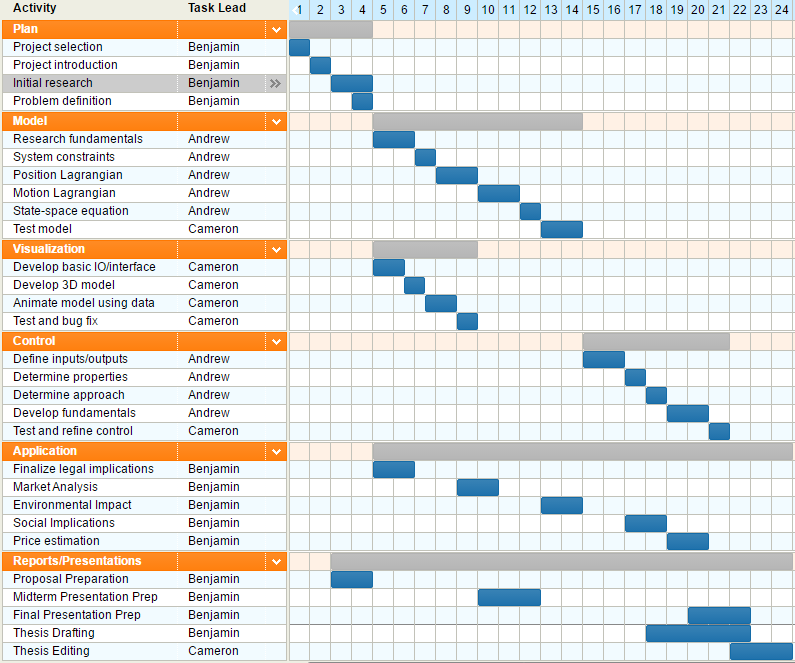
\includegraphics[width=\linewidth]{Gantt_Chart.PNG}
\caption{Full project timeline, with week number along the horizontal axis }\label{fig:gantt}
\endminipage
\end{figure}

\clearpage
\subsection{Task List}
Table 2 summarizes the tasks shown in Figure \ref{fig:gantt} with increased detail where necessary
\begin{center}
\textit{\textbf{Table 2:} Task list with estimated timeline for project deliverables, grouped by deliverable}
  \begin{tabular}{|p{2.3cm}|p{10.5cm}|p{2cm}|}
    \hline
    \textbf{Deliverable} & \textbf{Task} & \textbf{Timeline} \\ \hline Visualization &
Develop basic IO and interface for visualization tool & 1.5 weeks\\ \hline Visualization &
Develop 3D Ripstik model for visualization tool & 1 week\\
 \hline Visualization &
Animate model using model output & 1.5 weeks\\
\hline  Visualization &
Final testing and bug fixing & 1 week\\
\hline Model &
Research and learn the fundamentals of Lagrangian mechanics & 2 weeks\\ \hline Model &
Define and mathematically represent the system constraints & 1 weeks\\
\hline Model &
Develop the Lagrangian for the position of the Ripstik & 2 weeks\\
\hline Model &
Develop the Lagrangian for the motion of the Ripstik & 2 weeks\\
\hline Model &
Create a state-space equation that accurately models the Ripstik & 2 weeks\\


\hline Model &
Test, verify and fix model & 2 weeks\\
\hline Control &
Clearly define the inputs and outputs of the control system & 2 weeks\\
\hline Control &
Determine properties of the control system & 1 weeks\\
\hline Control &
Research viable control system approaches for the given system properties & 1 week\\

\hline Control &
Develop control system fundamentals & 2 weeks\\

\hline Control &
Test and refine control system based on evaluation requirements & 2 weeks\\
\hline Application &
Finalize the legal and ethical implications of the model and control system & 2 weeks \\
\hline Application &
Develop an extensive economic market analysis for the proposed application & 2 weeks\\
\hline Application & 
Establish the environmental impact of the materials required for the proposed application & 2 weeks\\
\hline Application &
Develop an accurate price estimate for the proposed application & 2 weeks\\
\hline Application & Establish the social implications associated with the proposed application, with a focus on safety considerations & 2 weeks\\
\hline
\end{tabular}
\end{center}
\clearpage